% This is latex template version 0.1
\documentclass[twosided,times,11pt]{article}

\usepackage[draft]{djb}
\usepackage{shortcuts}
\usepackage{fancyhdr}

%%%%%%%%%%%%%%%%%%%%%%%%%%%%%%%%%%%%%%%%
%%% Scribes: you must fill these in %%%%
%%%%%%%%%%%%%%%%%%%%%%%%%%%%%%%%%%%%%%%%
\newcommand{\lecdate}{November 23, 2011}
\newcommand{\lectitle}{A Taxonomy of Vulnerabilities In Differential GPS}
%%%%%%%%%%%%%%%%%%%%%%%%%%%%%%%%%%%%%%%%


\pagestyle{fancyplain}

\setlength{\headheight}{14pt}
\lhead[\fancyplain{}{\bfseries \thepage}]%
      {\fancyplain{}{\bfseries\lectitle}}
\chead[]{}
\rhead[\fancyplain{}{\bfseries\lectitle}]%
      {\fancyplain{}{\bfseries \thepage}}
\lfoot[{\small\scshape Project Writeup}]{{\small\scshape Project Writeup}}
\cfoot[]{}
\rfoot[{\small\scshape\lecdate}]{{\small\scshape\lecdate}}

\hypersetup{%
pdfauthor = {Brady Tello},
pdftitle = {\lectitle},
bookmarksopen= {true}
}

\begin{document}
\maketitle

\section{Introduction}

// TODO Introduce GNSS

\section{Differential GPS}

Differential GPS or DGPS is a method for increasing the accuracy of ordinary
GPS.  Several factors contribute to error in GPS with a single receiver.  These
include ionospheric refraction of the GPS signal, noise, clock errors, and other
sources.  The idea behind DGPS is that a second receiver called a reference
station is placed in a known location and can measure the error between
the expected signal and the signal actually received.  The reference station
then transmits this difference to the roving receiver, which applies the
information to its position calculation.  The result is a more accurate
position calculation for the rover.  Applying DGPS to ordinary GPS can cause
the accuracy to improve from about 15 meters of error to about 2-3 centimeters
of error. [Evan7], [Evan8]

DGPS is a term that applies to all types of GPS that have two or more receivers
for more accurate readings, but can be broken down into two categories.
DGPS is usually the term usually applied to the types of Differential GPS that
obtain meter level accuracy of readings.  Kinematic GPS, such as Post-Processed
Kinematic GPS and Real-Time Kinematic GPS are a different kind of DGPS that
can obtain accuracy within the centimeter level.

Kinematic GPS and DGPS share the same idea of using two receivers, but are
different in many ways.  Kinematic GPS takes about a minute to initialize and
requires five satellites to work properly.  This is compared to the instant
initialization of DGPS and the three to four satellites required to function.
Kinematic GPS measures differences in the high frequency carrier wave of GPS
to determine centimeter level accuracy as opposed to DGPS which uses the lower
frequency code phase methods for obtaining meter level accuracy.

\section{RTCM and Ntrip}

The Radio Technical Commission for Maritime Services (RTCM) is a non-profit organization comprised of both government and non-government bodies that publishes standards related to several topics including differential GNSS.   RTCM�s Special Committee 104 publishes two standards which we focused on in our research.  

First we will discuss the RTCM 10403.1 standard (Differential GNSS Services Version 3).  The 10403.1 standard defines a set of messages which contain the data required by Differential GNSS capable receivers\cite{RTCM3}.  The data defined by this standard is commonly referred to as just ``RTCM'', ``RTCM-104'', or ``RTCMv3''.  From this point on, we will refer to the data standard as RTCM unless it would be ambiguous in which case we will be careful to clarify the intended meaning.
\newline

\begin{figure}[h!]
	\centering
		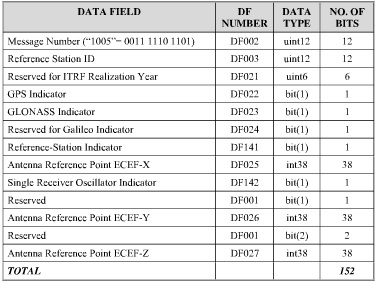
\includegraphics[scale=0.60]{RTCM1005.jpg}
	\caption{An Example of an RTCM Message}
\end{figure}

The second standard of interest is known as Ntrip (Networked Transport of RTCM over Internet Protocol) which is also published by the RTCM Special Committee 104.  Ntrip is an application layer networking protocol designed to stream RTCM correction data over the Internet.  A feature of Ntrip that seems to be popular is that it can transmit corrections over cellular data networks such as GPRS and EDGE, thus allowing corrections to be downloaded in very remote locations.  After conducting a survey of commercial GNSS devices and conducting brief interviews with sources close to the development of Ntrip we have come to the conclusion that most commercial GNSS reference stations are equipped with the capability to transmit RTCM correction data over Ntrip.  Furthermore, it has a wide variety of use cases which will be discussed in Section 4. The technical details of the protocol are contained in the following paragraphs.

The primary objective of the Ntrip protocol is to transmit correction data from reference stations to receivers over the Internet.  Its architecture is similar to that of a streaming Internet radio service.  When a GNSS receiver wants to ``listen'' to a correction stream from a reference station, it requests the stream from a broadcast source which delivers the stream to the receiver in real time.  In Ntrip terminology a reference station is known as an Ntrip Source, a receiver is known as an Ntrip Client, and a broadcaster is known as an Ntrip Caster.  An additional component known as an Ntrip Server acts as a middle man between sources and casters.  The server aggregates data streams coming from sources and delivers them to casters which in turn aggregate several servers.
\newline

The standard is relatively abstract in its definitions of these components so it is helpful to understand how they might be implemented in a real Ntrip network.  An Ntrip source is simply a pseudonym for a GNSS reference station such as the Trimble NetRS on which we conducted our experiments.  The device generates raw RTCM data which is uploaded to a server using one of several communications interfaces such as serial, TCP/IP, or various others (the Ntrip standard actually doesn�t define a communication interface between sources and servers).  An Ntrip Server and an Ntrip Caster are generally implemented as traditional software packages installed on one or more desktop/laptop computer(s).  Although they are defined as two logically separate entities, the server and caster can be implemented as part of the same program and still conform to the specification \cite{NTRIP2}.  A client is a piece of software at the end users receiver which is trying to correct its position.  A client downloads a list of reachable devices from the caster.  The list of devices is called a source table and contains entries for other casters, networks, and correction streams.  The Ntrip client downloads corrections and hands them off to the GNSS software which then applies them to an uncorrected position in order to get a corrected, high precision, position. During our research we have found Ntrip client programs implemented on cell phones and devices known as data controllers, however, it would be perfectly reasonable to implement it directly on the receiver itself.


\begin{figure}[h!]
	\centering
		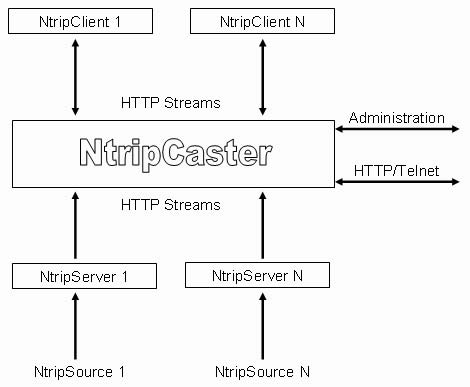
\includegraphics[scale=0.60]{ntripdiagram.jpg}
	\caption{Ntrip Protocol Architecture}
\end{figure}


The reason we have decided to focus our efforts on Ntrip and RTCM is because of their non-proprietary nature.  The two are not the only protocols available for encoding and disseminating differential correction data but they are certainly widely implemented and open to the general public (for a small fee).  Knowing that all differential GNSS packages adhere to the same physical principles, we assume that they would be vulnerable in similar ways but this question is left for future work.

\section{Sample Applications}

This section will enumerate a subset of the possible applications of differential GPS.  The applications listed here are those for which we were able to determine that Ntrip is being used in some way.  One should refer to the National DGPS Assessment Report from the US Department of Transportation\cite{NDGPS1} for a more comprehensive list of the application domains of GNSS in general.

\subsection{Machine Control}

Machine control is a sector of the GNSS industry which aims to make construction projects more efficient and accurate.  In machine control, GNSS receivers are hooked up to construction equipment such as bulldozers, scrapers, excavators, etc.  The GNSS receivers assist equipment operators in things like maintaining consistent grades throughout a project.  For example, if a grader were too far off its mark, the GNSS system could either warn the operator or make automatic corrections without operator assistance.  This saves time and money for a construction firm and would most likely increase the overall quality of their work.  By using differential GNSS techniques,  the equipment can be made even more accurate \cite{TRIMBLE_MACH_CTRL}.

\subsection{Navigation}

Real time maritime and aerial navigation are two applications which are especially interesting.  During the course of our research, we were unable to find any specific instances of Ntrip in use in either arena.  We do know, however, that the NetRS device can be configured to function as a Wide Area Augmentation System (WAAS) reference station.  Since we have shown that the NetRS is vulnerable to compromise, this probably isn't a good thing.  The NDGPS assessment report contains an excellent list of real world applications of Differential GNSS in the navigation domain \cite{NDGPS1}.

Automating your steering wheel is another interesting area in which high precision GNSS could be used.  In \cite{Uradzinski:2010}, the use of Ntrip based RTK solutions was investigated for its use in automated collision avoidance for land based automobiles.  While this was only a research study, it shows that there are people who are interested in applying this technology to automated land based vehicle navigation.  Another example of such a system is the Cooperative Intersection Collision Avoidance System (CICAS) run by the US Dept. of Transportation and described in \cite{NDGPS1}

\subsection{Surveying}

Surveyors, by the nature of their profession, require the use of very precise position information and thus benefit greatly from the use of differential GNSS technologies.  Surveyors often perform the task of staking out important geographical reference points.  To get an idea of the importance of the accuracy of reference points, imagine trying to build a house based on a reference point that was off by a foot.  If you didn't catch the mistake, your entire house would be shifted a foot from where you wanted it!  While, admittedly, this is a contrived example, it is simply meant to illustrate the types of errors that can occur if a surveyor is wrong.  The work of surveyors is broad in scope but it is fair enough to say that they are responsible for laying the basis for geographic measurements within a given context.  If they are wrong, everyone else will be wrong as well.

\subsection{Infrastructure Monitoring}

Monitoring of critical infrastructure such as bridges, tunnels, and dams is an important part of the professional surveying community.  Infrastructure monitoring involves installing high precision sensors in strategic locations on structures of interest.  The sensors generate position data which is compared against a set of movement thresholds.  If the thresholds are broken (the structure has shifted an unacceptable amount) a notification is delivered so that appropriate action can be taken\cite{TRIMBLE_INF_MON}.

\subsection{Early Warning Systems}

The University of California San Diego maintains a real time GNSS network dedicated to researching ``early warning systems for natural disasters'' \cite{UCSD_RTN}.  The network is known as the California Real Time Network.  A brief survey of some of the documents found on the network's website indicate that the primary concern is earthquakes.

\section{Attack Vectors}

In this section, we will outline potential attack vectors against Ntrip networks.  These are mechanisms by which an attacker can influence the data received by an Ntrip client.  A list of objectives of these attacks is provided in Section 6.

\subsection{Security Statistics}
To assist us in our attack vector assessment, we have collected a small body of statistics regarding the security of Ntrip sources.  We wrote a script which scanned the list of casters provided at rtcm-ntrip.org to determine what kind of security is in place in the wild for Ntrip sources.  

Our script considered the Ntrip network as a directed cyclic graph with a ``root'' vertex at rtcm-ntrip.org which provides links to over 140 Ntrip casters\cite{NTRIP_BC_INFO} (22 of which we were unable to connect to).  The source table obtained from a vertex describes the edges leading to neighboring vertices.  Caster, and network entries in a  vertex's source table are considered branch nodes and source entries are considered leaves.  

The script we wrote performed a traversal to depth 1 in the graph, gathering statistics about each Ntrip source encountered including: device type, whether a fee is charged for accessing the source, and whether the device uses digest or basic authentication.  We chose to only go to depth 1 in the interest of time.  This gave us statistics on over 5000 source devices.  What we found is that only one of the streams required digest authentication, 867 of them assessed a fee, and that the Trimble NetRS was the most prevalent device found in the wild (22 percent of the devices we found were NetRS stations).

It should be noted that although this is a fair amount of data, it is likely only a small sampling of the total population of Ntrip sources.  Our script identified 291 caster links which it simply ignored.  Since we only scanned 119 casters, one can imagine how much data is still available.   

// TODO Insert some sort of chart summarizing the important security statistics (Should be able to generate one from the SourceStatistics.xls file contained in the repo)

\subsection{Man in the middle}

The most serious attack vector we have identified is a man in the middle attack between casters and clients.  If a skilled adversary could convince a client to connect to his malicious caster using any number of network based man in the middle attack tools such as the freely available Cain and Abel or the GRPS, EDGE, UMTS, HSPA targeted attack described in  \cite{BLACKHAT:2011}  he could easily spoof the Ntrip protocol and trick the client into using corrupted correction data.  This attack is possible due to the lack of mutual authentication between clients and casters in the Ntrip protocol.

We consider this the most dangerous of our attacks because it is equivalent to compromising the RTCM streams served by that caster.  This way, an attacker wouldn't have to worry about the receiver device ``averaging out'' a misbehaving stream (so far we have found no evidence of software that does this) as long as they spoofed all the streams to  misbehave identically.

\subsection{Authentication Spoofing}  

Authentication is used in Ntrip networks to access RTCM streams or administer casters/servers \cite{NTRIP1} \cite{NTRIP2}.  If an attacker can determine a valid set of credentials they could either access restricted services (described in the false billing section) or configure a caster/server in a malicious manner.

The Ntrip standards do not specify exactly how a caster/server must be implemented but they do state that administrators are responsible for registering devices with casters/servers.  If an attacker were to gain access to the administration interface he could register malicious servers with a legitimate caster or malicious sources with legitimate servers (which would propagate to the caster and client).

Casters have the option of specifying basic or digest authentication methods for accessing sources.  An initial thought was that we would have to find a way to crack digest authentication in order to access the sources.  After analyzing the results of our scan however, it is clear that this isn't really necessary in the vast majority of cases (assuming that our sample data is representative of the entire population).  Only a single stream out of nearly 5000 was protected by digest authentication.  A wise attacker would obviously reach for the low hanging fruit and simply monitor the network to obtain the base64 encoded credentials which can be trivially decoded using any number of web/client based tools.  We ran a Base64 decoder on the encoded credentials transmitted by a reference implementation of an Ntrip client and verified that the plaintext credentials are trivially retrieved.

Regarding the caster/server passwords we can't say how difficult it would be to obtain a set of credentials in every case.  The first Ntrip standard specifies that caster administration is performed using telnet which would be an easy target but the second version does not specify the exact administration method.  It is thus our recommendation that implementors choose a sufficiently secure authentication method in order to prevent against this type of attack.

\section{Attack Taxonomy}

 \subsection{Economic Damage}
 
 Almost all of the attack objectives outlined in this section will cause some level of economic damage.  An attacker could destroy automatically piloted vehicles, cause faulty surveys resulting in wasted effort or damage to structural integrity, make false charges to an Ntrip subscribers account, etc.
 
Lax security in differential GNSS means that the high precision guarantees might not be guarantees at all.  If enough people were to catch on to this fact, the entire industry could suffer as a result.

\subsection{Navigational Control Hijacking / Confusion}

In our attack against a reference RTK implementation described in Section 7, we have found that it is possible to control a receiver's position calculations with some degree of accuracy.  This is possible by spoofing the reported X and Y coordinates of a reference station in message 1005 of the RTCM3 stream.  If a concrete receiver implementation exhibited similar behavior, it would be possible to control automated navigation systems that use Ntrip.  For example, if a receiver were reporting positions that were 1 foot to the West of its actual location, any software using this data to correct its position would adjust its course 1 foot to the East.  This attack could be used to confuse or even control automated navigation systems.

\subsection{False Billing} 

Depending on the billing model used, an attacker could log excessive accesses to a legitimate user's account.  The billing models we encountered were all flat rate charges (per month) but one could imagine other pay-per-use systems.  For example, if a service provider charged a dollar for every MB of correction data downloaded, an attacker could cause financial damage to a subscriber.

\subsection{Diversionary Attacks}

The use of differential GPS in infrastructure and environmental monitoring projects provides an interesting diversionary attack\cite{UCSD_RTN}.  Say an attacker wanted to destroy a bridge on the East side of a city without alerting authorities of his presence.  He could cause a monitoring device to report structural damage to a bridge on the west side of that city while suppressing alarms from the bridge being destroyed.  Depending on the level of response to such an alarm, authorities and resources would be diverted to the site of the false damage in the West while the attacker wreaked havoc in the East.  This is similar to Stuxnet's method of causing critical warning mechanisms to report that the system was performing normally\cite{STUXNET}. 

\subsection{Location Privacy Violations}

Section 2.1.3 of the Ntrip version 2 standard describes functionality in which a client transmits its location information to a caster so that the caster can provide location aware services.  An attacker who can monitor the network or who has control of a caster can thus observe the position of a client which may not be acceptable in certain circumstances.

\section{An Attack on a Real Time Kinematics Engine}

\begin{center}
	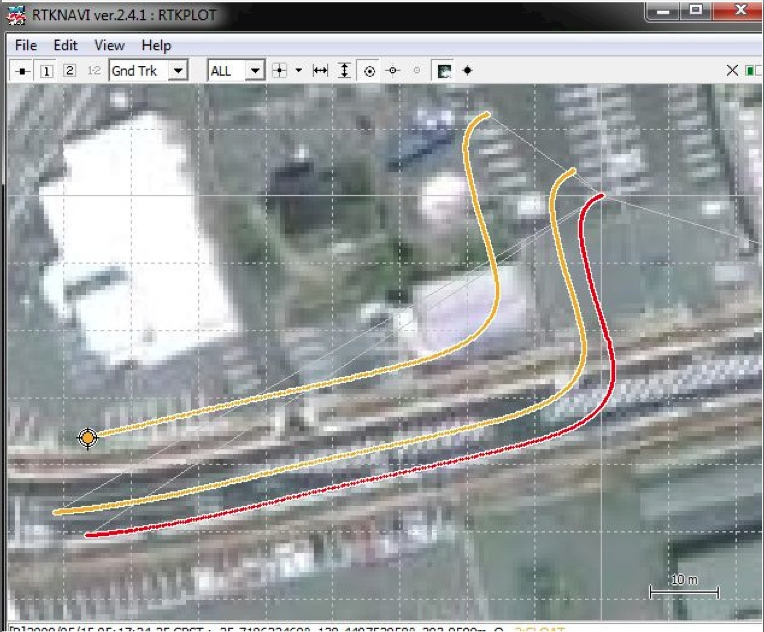
\includegraphics[scale=0.4]{controlledShiftUsingRTCM1005.jpeg}\\
\end{center}

\subsection{Attack Testbed}

Before we go into details of the attack on a Real Time Kinematics Engine, we will first describe the testing environment we used.

\begin{figure}[h!]
	\centering
		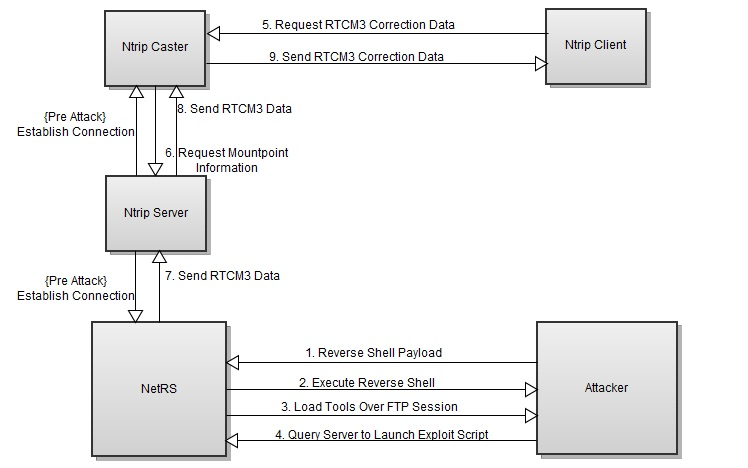
\includegraphics[scale=0.50]{attack-diagram.png}\\
	\caption{Attack Diagram}
\end{figure}


In order to show how our attack works, we needed to set up an environment eqivalent to that of a fully functioning Ntrip network.  We set up a Linux virtual machine running an FTP server and a reference implementation of a caster and server which was downloaded from BKG's official Ntrip site\cite{NTRIP_BC_INFO}. The Windows 7 host machine was running an Ntrip Client.  We connect to the NetRS device over a TCP/IP connection through the Linux virtual machine.

\subsection{The Attack}

The Ntrip Client in our test environment receives RTCM3 correction data and applies that correction data to the GPS stream it normally receives.  The client will recalculate where it believes it is located based on this correction data.  The Ntrip Client will query an Ntrip Caster and request correction data from a specific mountpoint that the Ntrip Caster knows about.  The Ntrip Caster receives information about its associated mountpoints through an Ntrip Server.  The Ntrip Server connects to its associated mountpoints to receive streaming correction data that it forwards to the Ntrip Caster.  For the purposes of our attack scenario, the mountpoint the client is requesting updates from is the compromised NetRS device.

To setup our attack scenario we configure an Ntrip Caster and an Ntrip Server to communicate together.  The Ntrip Server is configured to receive streaming data from the NetRS device and to forward that data to the Ntrip Caster.  The Ntrip Caster is configured to receive mountpoint information from the Ntrip Server and to forward the correction information for a given mountpoint to a client that has the proper credentials, username: user and password: prettyplease.

First, we must compromise the NetRS device in our attack.  The NetRS runs an Apache web service for remote access to the NetRS machine.  By launching a carefully constructed payload against the NetRS, we gain a reverse shell to the NetRS device.  We can then upgrade our privileges to root and set the associated partition we want to load our tools to as writeable.

The NetRS device does not contain many precompiled programs, e.g. Python interpreter, Perl interpreter, whoami, emacs, etc, and is running on a PowerPC architecture.  The NetRS does have the FTP program, and we load our exploit script by connecting to the running FTP server on our attack machine and sending the script over the TCP/IP connection.  Also, the Apache web service runnning on the NetRS can run perl programs meant for CGI scripts rather than just having a Perl interpreter.  In order to avoid cross-compilation issues and to simplify the attack, we use the Apache web service to run our custom perl exploit script.

Our exploit script acts as a normal Ntrip Source that sends out RTCM3 correction data.  In our attack, we customize the RTCM3 stream of data to correct positions to six meters off of its normal location.  We launch the perl server by sending a query to our perl script via the webserver and establish a connection to the NetRS device with the Ntrip Server.  The Ntrip server receives the correction stream and updates the associated mountpoint in the Ntrip Caster.  When the Ntrip Client connects to the Ntrip Caster and asks for correction data about the compromised mountpoint, the client receives correction data that is six meters off of its actual location.  The client accepts this information and recalculates its position to be six meters off of its actual location.

\subsection{Attack Mitigations}

The Ntrip network should be resilient to attack for reliable GPS correction data.  NDGPS uses a reference monitor to check the network for correction data outside of a given normal value.  Ntrip could potentially use a similar monitoring system to ensure the correction data traveling from an Ntrip Source propagating to an Ntrip client is within a valid range.

All authentication traffic should be encrypted.  Allowing passwords to be transmitted in plaintext or base-64 encoding should be eliminated from the Ntrip system.  Also, mutual authentication should occur between entities in the Ntrip network to thwart Man in the Middle attacks.

Future research should include additional research into attack mitigations as well as their effect on the Ntrip network.

\section{Scope of Impact}

Both the attack created in this research as well as the other attacks mentioned
show the high level of vulnerability in DGPS.  Anyone with knowledge of these
attacks could remotely manipulate DGPS information around the world.
Therefore, any application that relies on DGPS is at risk of receiving
incorrect location information at any time.  This could have far reaching
effects on many people.  The results could range from a loss of time and money
to physical danger and human death.

The attack outlined in this paper was crafted specifically for the Trimble
NetRS reference station, and as such the results are limited to that device.
However, the Trimble NetRS is the most widely deployed Reference Station
that can be found through the master NtripCaster list on rtcm-ntrip.org.
Out of 4995 Reference Stations, 1126 were Trimble NetRS devices, vulnerable
to the attack outlined in this paper.  [Evan6]

Further digging also shows that the sources in the field are indeed vulnerable
in other ways as well.  Out of the 4995 reference stations, 4994 use basic
authentication with nothing more than base-64 encoding to protect username
and passwords.  Only one reference stations uses the stronger digest
authentication to provide any protection from snooping passwords.  [Evan6]

There are many applications that use DGPS.  Here are a few:
(TODO Actually, these are the propused uses of NDGPS. Make sure these
are actually used)
-Positive Train Control
-Precision farming and agriculture
-Smart Vehicles
-Snow Plow Management
-Accurate Waterway Dredging
-Emergency Response
---------------------------------------------------------
-Maritime harbor/harbor approach navigation
-Vessel tracking
-Buoy positioning
-Surveying
-National Spatial Reference System
-Ionospheric monitoring
-Weather prediction research
-Monitoring of large structures such as bridges and dams
[Evan1], [Evan2], [Evan3], [Evan4], [Evan5]

In the case of farming and agriculture, corrupted DGPS data might cause
farmers to inefficiently lay out crops or affect irrigation methods that may
cause crops to die.  Irrigation drip tape must be laid with inch level
accuracy to effectively water crops.  This would result in lost time and money.
[Evan7]

\textbf{Integrity Monitor Stuff}

\section{Future Work}

Investigate how networks average error
Find out if the corrupted corrections can be used to affect time calculations
Investigate other DGPS protocols
Run our attack on a real RTK receiver (not rtklib)  and see if we get similar results

\section{Conclusion}

We have discovered a Diffierential GNSS system that is widely used yet highly insecure.  It is important for all users and implementors of differential GNSS technologies to make security more of a priority as cyberphysical security is an area of active research and interest.

\section{Thanks}

Dr. Georg Weber for providing helpful links and commentary on the adoption of Ntrip in geodetic equipment.
Jeff Jalbrzikowski for providing valuable guidance regarding real life applications of Differential GPS and GNSS in the context of Surveying.
Tyler Nyswander for sharing his efforts in gaining root access to the NetRS device.

\bibliographystyle{plain}
\bibliography{biblio}

\end{document}


